\chapter{Building large SpiNNaker machines}
	
	When physically constructing a large super computer the network topology used
	can have a huge impact on the cost, complexity and effort involved in the
	process. This chapter describes the approaches used to design conventional
	torus-based super computer installations which ensure that cable lengths
	remain manageable and ensure a technician is realistically able to connect
	them. These approaches, unfortunately, do not extend directly to hexagonal
	torus topologies and so a number of new techniques are described which allow
	large hexagonal-torus based systems to be constructed. The chapter concludes
	by describing the successful application of these techniques to very large
	SpiNNaker machines.
	
	\section{Related work}
		
		The process can be broken into three steps: partitioning, layout and
		installation. During partitioning the topology is broken up into pieces
		which can easily be manufactured and handled. During layout, the
		partitioned pieces of the topology are physically laid out in order to
		control cable length. During installation a technician must physically
		install cables connecting things together.
		
		\subsection{Partitioning hexagonal toruses}
			
			The nodes in most super computer networks are relatively fine-grained by
			comparison with their physical construction in order to make construction
			more practical. For example, a single circuit board may contain tens or
			even hundreds of nodes \cite{gilge14,ajima12}. The majority of commercial
			super computers use torus topologies partitioned into hypercubes as
			illustrated in figure \ref{fig:hypercube-partitioning}
			\cite{chen11,ajima12}.
			
			\begin{figure}
				\center
				\begin{subfigure}[b]{0.45\textwidth}
					\center
					\buildfig{figures/hypercube-partitioning.tex}
					\caption{2D hypercube partitioning}
					\label{fig:hypercube-partitioning}
				\end{subfigure}
				\begin{subfigure}[b]{0.45\textwidth}
					\center
					\buildfig{figures/parallelogram-partitioning.tex}
					\caption{Parallelogram partitioning}
					\label{fig:parallelogram-partitioning}
				\end{subfigure}
				
				\caption{Conventional hypercube topology partitioning (a) and the
				hexagonal torus topology analogue (b).}
				\label{fig:partitioning-options}
			\end{figure}
			
			One possible analogue in a hexagonal torus topology is a parallelogram as
			illustrated in figure \ref{fig:parallelogram-partitioning}.
			
			Each partition connects to six neighbouring partitions and, unlike
			hypercube partitions, the number of connections to each is imbalanced.
			Specifically the partitions above-right and below-left are connected by
			only one link each. The consequence is potentially a need for multiple
			types of interconnect for connecting partitioned pieces of the system,
			adding both to design complexity and cost.
			
			Another `obvious' choice of partition is that of a hexagon wrapped in
			concentric layers of hexagons as illustrated in figure
			\ref{fig:wrapped-hexagon-tiling}.
			
			\begin{figure}
				\center
				\buildfig{figures/wrapped-hexagon-tiling.tex}
				
				\caption{A single hexagon wrapped in layers of hexagons does not tile the
				same way as a pointy-topped hexagon.}
				\label{fig:wrapped-hexagon-tiling}
			\end{figure}
			
			While this partition presents six equally-sized edges, it cannot be used
			to build a hexagonal torus as described. A partition constructed from
			pointy-topped hexagons tiles a hexagonal torus topology constructed from
			pointy-topped hexagons iff the partition tiles with a translational
			symmetry shared with a hexagonal torus. As we can see from the figure,
			this is not the case. This tiles more like a twisted torus of some sort.
			To prove this test is legit, see figure \ref{fig:parallelogram-tiling}
			where we superimpose a pointy-topped hexagon on a parallelogram.
			
			\begin{figure}
				\center
				\buildfig{figures/parallelogram-tiling.tex}
				
				\caption{Demonstration that a parallelogram partition tiles a hexagonal
				torus.}
				\label{fig:parallelogram-tiling}
			\end{figure}
			
			Furber, Davison \emph{et al.} \cite{davidsonWiring} proposed an
			alternative based on wrapped triples where you take three hexagons and
			wrap more layers around them as required. This pattern tiles like
			flat-topped hexagons, which isn't quite right. But since we know a
			pointy-topped triple tiles like a flat-topped hexagon, a flat-topped
			triple must tile like a pointy-topped hexagon. Combining these facts
			gives that by tiling triads of wrapped triples we can tile a hexagonal
			torus.
			
			\begin{figure}
				\center
				\buildfig{figures/wrapped-triple-tiling.tex}
				
				\caption{Three pointy-topped hexagons tiles in the same way as flat-topped
				hexagons.}
				\label{fig:wrapped-triple-tiling}
			\end{figure}
			
			\begin{figure}
				\center
				\buildfig{figures/triad-tiling.tex}
				
				\caption{Demonstration that a triad tiles a hexagonal torus topology.}
				\label{fig:triad-tiling}
			\end{figure}
		
		\subsection{Folding regular toruses}
			
			Once partitioned, a na\"ive arrangements of torus topologies, including
			hexagonal torus topologies, feature long `wrap-around' connections. In
			conventional torus topologies these long connections are eliminated by
			folding and interleaving nodes of the network. For example, for a 1D
			torus network (a.k.a. a ring network), one long connection exists to
			connect the two opposite sides of the system. To remove these long
			connections, half the nodes are `folded' on top of the others and then
			this arrangement of nodes is interleaved.
			
			\begin{figure}
				\center
				\begin{subfigure}[b]{0.39\linewidth}
					\center
					\buildfig{figures/ring-folding-row.tex}
					\caption{A ring network}
					\label{fig:ring-folding-row}
				\end{subfigure}
				\begin{subfigure}[b]{0.24\linewidth}
					\center
					\buildfig{figures/ring-folding-folded.tex}
					\caption{Folded}
					\label{fig:ring-folding-folded}
				\end{subfigure}
				\begin{subfigure}[b]{0.35\linewidth}
					\center
					\buildfig{figures/ring-folding-interleaved.tex}
					\caption{Folded and interleaved}
					\label{fig:ring-folding-interleaved}
				\end{subfigure}
				
				\caption{Folding and interleaving a ring network to reduce maximum wire
				length.}
				\label{fig:ring-folding}
			\end{figure}
			
			This approach substantially decreases the maximum wire length (in fact
			does so regardless of network size) at the expense of approximately
			doubling the average wire length. In practice, the maximum length is more
			important and so this approach is widely used in practice.
			
			Unfortunately, the non-orthogonality of hexagonal torus topologies means
			that folding does not work correctly. In this chapter I describe a few
			transformations that fix this in various settings.
		
		\subsection{Cabling installation}
			
			Existing machine room installations feature very repetitive cabling
			patterns which can easily be memorised by a human technician.  For
			example in BlueGene super computers connectivity between neighbouring
			racks are highly regular \cite{lakner07} and in data centre networks
			cabling often centres around a small number of high-port-count switches
			\cite{cisco07,csernai15}.
			
			Like many super computers and some new data centre network architectures
			\cite{abu11}, SpiNNaker features point-to-point connectivity between
			compute nodes rather than relying on external network switching hardware,
			typically resulting in greater cabling complexity. Due to the small scale
			and high packing density of SpiNNaker's compute nodes the cabling
			complexity is further exacerbated.
			
			Cable installation is usually only aided by the labelling of connectors
			and sockets using widely used in data centres \cite{tia2006} and super
			computers such as BlueGene (see figure \ref{fig:bgWiring}).
			
			\begin{figure}
				\center
				\begin{subfigure}[t]{0.5\textwidth}
					\begin{tikzpicture}
						\node (cables) [inner sep=0]
						      {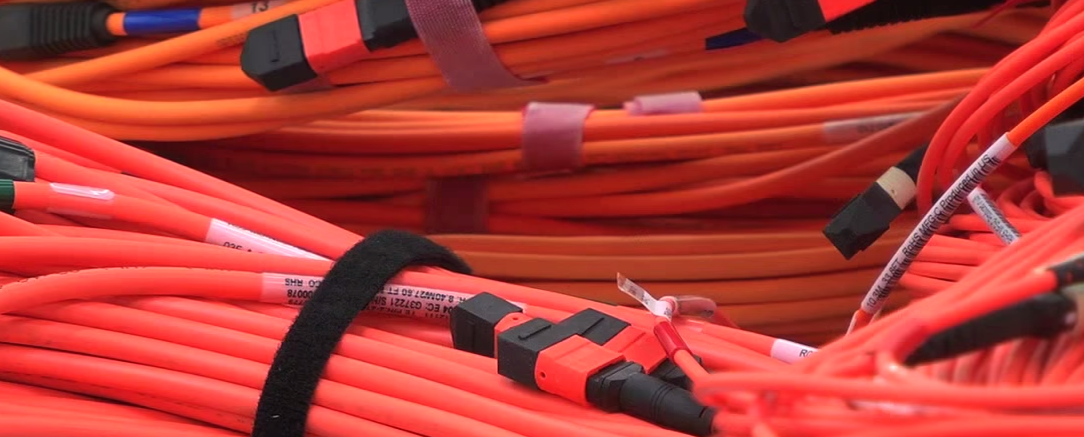
\includegraphics[width=\textwidth]{figures/bgCables.png}};
						\node (sockets) [inner sep=0, below=1.0em of cables]
						      {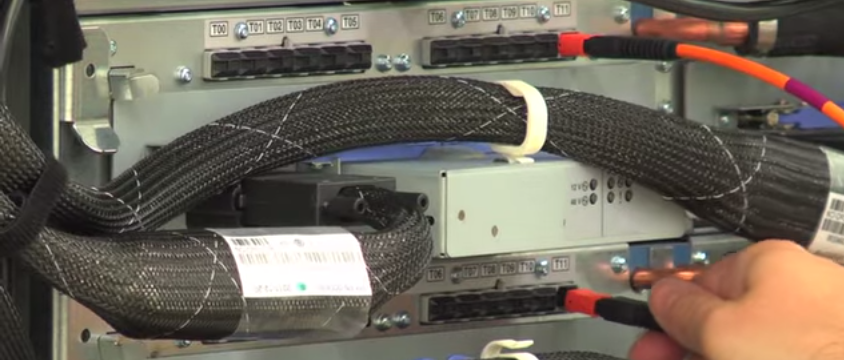
\includegraphics[width=\textwidth]{figures/bgSockets.png}};
						
						% Point at label on cable
						\draw [white, <-, line width=0.4em]
						      ([shift={(0.7cm, -0.3cm)}]cables.center)
						      -- ++(45:1cm);
						
						% Point at label on socket
						\draw [white, <-, line width=0.4em]
						      ([shift={(-1.0cm, 1.1cm)}]sockets.center)
						      -- ++(-45:1cm);
					\end{tikzpicture}
					
					\caption{Pre-labelled cables and sockets}
				\end{subfigure}
				~
				\begin{subfigure}[t]{0.30\textwidth}
					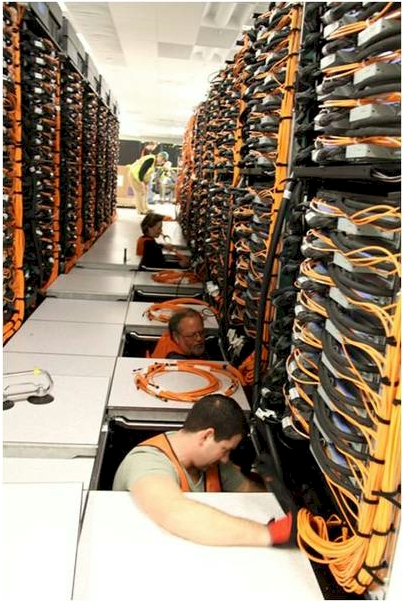
\includegraphics[height=6.15cm]{figures/bgWiring.jpg}
					
					\caption{Installation of cables}
				\end{subfigure}
				
				\caption{BlueGene/Q cable installation \cite{cscs13}}
				\label{fig:bgWiring}
			\end{figure}
			
			Despite the regularity and careful labelling of cables, installation and
			maintenance alone can be significant with costs in the range of \$45-95
			per 1 meter cable run and \$100-400 for runs of 10 meters
			\cite{mudigonda11}. Much of this cost is due to the care required during
			installation to avoid miswiring and ensure that cooling airflow is not
			hampered by cable runs \cite{cisco07}.
			
			Existing work to reduce cable installation costs have focused on
			developing alternative network topologies with shorter, or fewer, cable
			runs \cite{curtis12, popa10, mudigonda11}. By contrast, in this chapter I
			take an alternative approach: providing interactive guidance to cable
			installers to enable complex wiring schemes to be followed quickly and
			without mistakes. I also demonstrate that, contrary to conventional
			wisdom, the more complex wiring schemes proposed do not negatively impact
			either system maintainability or cooling performance.
	
	\section{Folding \& interleaving hexagonal toruses}
		
		In order to fold a hexagonal torus topology we must transform it into a
		regular rectangular grid. In this section we break this process down into
		two steps: transformation from a parallelogram to a rectangle and
		uncrinkling. We propose two alternative transformations which can be
		applied to hexagonal torus topologies constructed out of triads of triples
		or to the basic torus topology.
		
		\subsection{Transformation}
			
			The hexagonal torus topology is most naturally drawn as a parallelogram
			(see left of figures). As described earlier, folding this just doesn't
			work since the ends don't meet. To make this foldable we must transform
			the network into a rectangle. We present two transformations to do this.
			
			The first transformation we describe is shearing. When shearing you
			distort the network to cause the X and Y axes to become orthogonal and
			the whole shape to become a rectangle. The down-side of this approach is
			that the Z dimension has been stretched and this distortion means that
			cables going in the Z direction will need to be $\sqrt(2)$ times longer
			than those going in the X and Y directions.
			
			The second transformation is slicing where we translate the left triangle
			of the parallelogram onto the opposite side forming a generally
			rectangular shape. This transformation has the advantage that it
			maintains distances in hexagonal meshes without distortion but sadly with
			wires criss-crossing which will cause some headaches later.
			
			\begin{figure}
				\center
				\begin{subfigure}[b]{0.32\linewidth}
					\center
					\buildfig{figures/hex-to-plane-node-native.tex}
					
					\caption{$7 \times 7$ node torus}
					\label{fig:hex-to-plane-node-native}
				\end{subfigure}
				\begin{subfigure}[b]{0.32\linewidth}
					\center
					\buildfig{figures/hex-to-plane-node-shear.tex}
					
					\caption{Sheared}
					\label{fig:hex-to-plane-node-shear}
				\end{subfigure}
				\begin{subfigure}[b]{0.32\linewidth}
					\center
					\buildfig{figures/hex-to-plane-node-slice.tex}
					
					\caption{Sliced}
					\label{fig:hex-to-plane-node-slice}
				\end{subfigure}
				
				\caption{Transformations of hexagonal toruses of nodes into a
				rectangular form. Thin lines show wrap-around links. (Pointy-topped)
				hexagons represent individual nodes.}
				\label{fig:hexToPlaneNode}
			\end{figure}
			
			\begin{figure}
				
				\begin{subfigure}[b]{0.32\linewidth}
					\center
					\buildfig{figures/hex-to-plane-native.tex}
					
					\caption{$4 \times 4$ triad torus}
					\label{fig:hexToPlaneNative}
				\end{subfigure}
				\begin{subfigure}[b]{0.32\linewidth}
					\center
					\buildfig{figures/hex-to-plane-shear.tex}
					
					\caption{Sheared}
					\label{fig:hexToPlaneShear}
				\end{subfigure}
				\begin{subfigure}[b]{0.32\linewidth}
					\center
					\buildfig{figures/hex-to-plane-slice.tex}
					
					\caption{Sliced}
					\label{fig:hexToPlaneSlice}
				\end{subfigure}
				
				\caption{Transformations of hexagonal toruses of wrapped triples into a
				rectangular form.  Thin lines show wrap-around links. (Flat-topped)
				hexagons represent a wrapped triple of nodes.}
				\label{fig:hexToPlane}
			\end{figure}
			
		\subsection{Uncrinkling}
			
			At this point we have two ways of getting into a rectangular arrangement
			but this still cannot be folded since the spacing of individual nodes
			does not evenly fill a regular 2D grid. For sheared systems of triads and
			for sliced systems of either kind, the arrays of hexagons contain
			crinkled columns and rows as illustrated below.
			
			\begin{figure}
				\center
				\begin{subfigure}[b]{0.44\linewidth}
					\center
					\buildfig{figures/uncrinkling-node-sheared.tex}
					
					\caption{$7 \times 7$ nodes, sheared}
					\label{fig:uncrinkling-node-sheared}
				\end{subfigure}
				\begin{subfigure}[b]{0.44\linewidth}
					\center
					\buildfig{figures/uncrinkling-node-sliced.tex}
					
					\caption{$7 \times 7$ nodes, sliced}
					\label{fig:uncrinkling-node-sliced}
				\end{subfigure}
				
				\vspace{1cm}
				
				\begin{subfigure}[b]{0.44\linewidth}
					\center
					\buildfig{figures/uncrinkling-sheared.tex}
					
					\caption{$4 \times 4$ triples, sheared}
					\label{fig:uncrinkling-sheared}
				\end{subfigure}
				\begin{subfigure}[b]{0.44\linewidth}
					\center
					\buildfig{figures/uncrinkling-sliced.tex}
					
					\caption{$4 \times 4$ triples, sliced}
					\label{fig:uncrinkling-sliced}
				\end{subfigure}
				
				\vspace{1em}
				
				\caption{Mapping rectangular arrangements of hexagons into a square
				grid. Thick lines show how layers of hexagons are uncrinkled.
				Annotations show how the relative positions of nodes and wrapped triples
				change after uncrinkling.}
				\label{fig:uncrinkling}
			\end{figure}
			
			By uncrinkling these columns or rows, a regular 2D grid arrangement is
			formed. In the figure, the numbered hexagons enumerate the different
			positions on the crinkle and those labelled alphabetically are those that
			immediately surround them. From this we can observe that uncrinkling
			largely preserves spatial locality but some distortion is introduced
			separating previously neighbouring nodes. For example, in C, the wrapped
			triples labelled `1' and `i' are neighbours before uncrinkling but are
			separated by a (Euclidean) distance of $\sqrt{5}$ afterwards. Note that
			the distortion introduced depends on what part of the crinkle is
			considered, for example `2' and `a' have distance 2 but are logically
			connected in the same way.
		
		\subsection{Folding}
			
			We now have a square, 2D grid with the usual patterns of connectivity:
			all very local except for the connections crossing from side-to-side and
			normal folding techniques can be used.
			
			\begin{figure}
				\begin{subfigure}{\linewidth}
					\center
					\buildfig{figures/folding-sheared.tex}
					\caption{$N \times M$ sheared systems and $N \times 2N$ sliced systems}
					\label{fig:folding-sheared}
				\end{subfigure}
				
				\vspace{1em}
				
				\begin{subfigure}{\linewidth}
					\center
					\buildfig{figures/folding-sliced.tex}
					\caption{$N \times N$ sliced systems}
					\label{fig:foldingSliced}
				\end{subfigure}
				
				\caption{Schematic illustrating elimination of long wrap-around links
				during folding. In each example a single link has been highlighted to
				aid in following the process.}
				\label{fig:folding}
			\end{figure}
			
			That is unless you used the slicing technique. If you've done this then
			you get criss-crossing streams of cables which folding will not remove,
			depending on the dimensions of the network.
			
			\begin{figure}
				\center
				\buildfig{figures/slicing-examples.tex}
				\caption{Patterns of wiring in sliced systems of various sizes.}
				\label{fig:slicedSizes}
			\end{figure}
			
			If you have Nx2N then you actually get normal crossing patterns and thus
			folding can be done as-per-normal.
			
			If you have NxN, though, it all goes wrong and you get criss-crossing.
			Such systems can be folded by doing a double vertical fold.
		
		\subsection{Interleaving}
			
			Interleaving is performed as illustrated earlier.
			
			TODO: MORE FULLY SPECIFY
		
		\subsection{Mapping to Cabinets}
			
			A simple linear allocation to cabinet locations.
			
			TODO: DESCRIBE ALGORITHM
			
			\begin{figure}
				\center
				\buildfig{figures/cabinetisation.tex}
				
				\caption{Mapping from 2D space to cabinets, frames and boards}
				\label{fig:cabinetisation}
			\end{figure}
			
			The result is a connection list like so...
		
	\section{Installation}
		
		Installation will be performed by a (team of) technicians and requires that
		all cables are connected correctly and connectivity tested. We use some
		automation and guidance provided by SpiNNer.
		
		\subsection{Cable selection}
			
			Controlling slack is critical to ensuring reliable and maintainable
			cabling installations. If cables are too tight, cables and connectors can
			become easily damaged and when too slack, the excess cable obstructs
			other cables and can easily become tangled and damaged \cite{cisco07}. It
			has been observed that when ready-made cables are employed technicians
			frequently over-estimate the cable lengths required preferring to use
			overly long cables for all connections \cite{mazaris97}. To solve this
			problem, the SpiNNer wiring guide software dictates the cable lengths to
			be used by an installer based the rule of (three-)thumbs according to
			Mazaris \cite{mazaris97}. This rule suggests that an ideal amount of
			slack is approximately that which can be wrapped around three fingers.
			Specifically, the shortest available cable is selected which ensures at
			least \SI{5}{\centi\meter} of slack.
			
			The SpiNNer tool allocates cables assuming all cables take a Euclidean
			straight-line path between the endpoints of the connection. The result is
			that wiring is not routed through dedicated cable management structures
			but is simply suspended by its connectors in front of the machine. As
			demonstrated later, this unconventional approach leads neither to cooling
			problems nor increased maintenance effort.
		
		\subsection{Interactive technician guidance and validation}
			
			While automated systems for validating cabling correctness are
			commonplace, these systems are typically used only after cabling has been
			completed \cite{lakner07}. SpiNNaker features a low-bandwidth system
			management bus which may be used to interrogate SpiNNaker's network
			hardware and control diagnostic LEDs prior to the installation of the
			main SpiNNaker network interconnect. Using these facilities I have
			constructed a tool which interactively guides a technician through the
			cable installation process, checking each cable is installed in
			real-time.
			
			The interactive wiring guide uses a GUI (figure
			\ref{fig:interactive-wiring-guide-gui}) to give a visual indication of
			the endpoints of the next cable to install and also the cable length to
			use. The centre of the display shows a `big-picture' perspective of the
			locations of the boards to be connected. The detailed views on the left
			and right indicate which of the six sockets on each board the cables
			should connect. In addition to the GUI, diagnostic LEDs on the SpiNNaker
			machine itself are illuminated to indicate which boards to connect
			(figure \ref{fig:interactive-wiring-guide-leds}). Finally, a
			Text-To-Speech (TTS) system is used to announce the cable type and
			location of each connection which in practice means that a technician
			rarely needs to refer to the GUI during installation.
			
			\begin{figure}
				\center
				\begin{subfigure}[b]{0.546\textwidth}
					\begin{tikzpicture}[thin, black!20!white]
						\node (screen) [inner sep=0]
						      {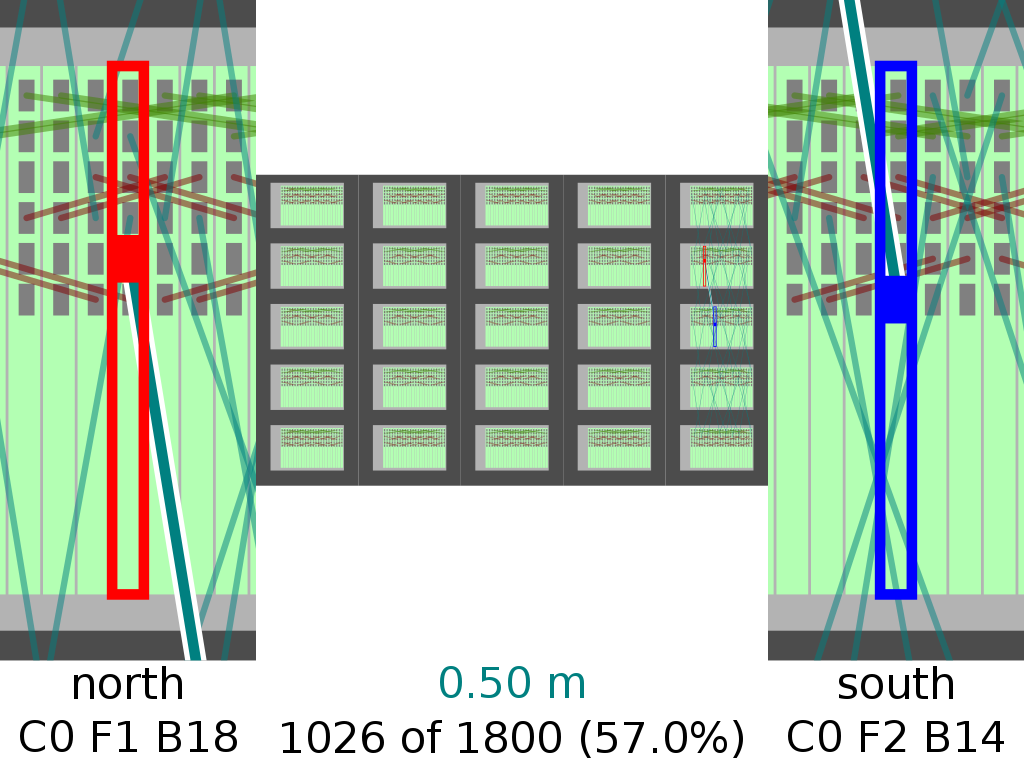
\includegraphics[width=\textwidth]{figures/wiring_guide_screenshot.png}};
						\draw (screen.south west) rectangle (screen.north east);
					\end{tikzpicture}
					
					\caption{Interactive wiring guide GUI}
					\label{fig:interactive-wiring-guide-gui}
				\end{subfigure}
				~
				\begin{subfigure}[b]{0.40\textwidth}
					\begin{tikzpicture}
						\node (leds) [inner sep=0]
						      {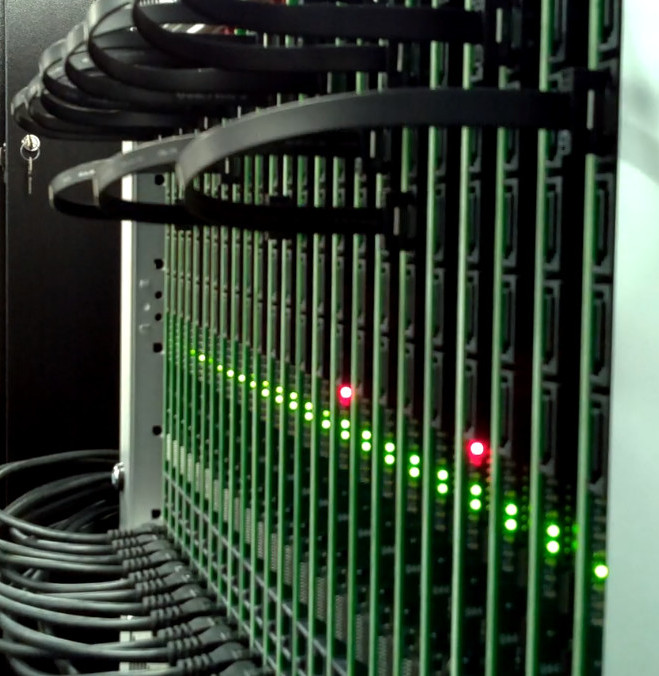
\includegraphics[width=\textwidth]{figures/leds.jpg}};
						% Point at left LED
						\draw [white, <-, line width=0.4em]
						      ([shift={(-0.0cm, -0.6cm)}]leds.center)
						      -- ++(225:1cm);
						% Point at right LED
						\draw [white, <-, line width=0.4em]
						      ([shift={(1.1cm, -1.1cm)}]leds.center)
						      -- ++(225:1cm);
					\end{tikzpicture}
					
					\caption{Diagnostic LEDs}
					\label{fig:interactive-wiring-guide-leds}
				\end{subfigure}
				
				\caption{The SpiNNer interactive wiring guide uses a GUI,
				text-to-speech and diagnostic LEDs to assist during cable
				installation.}
				\label{fig:interactive-wiring-guide}
			\end{figure}
			
			The interactive wiring guide also validates the connectivity of the
			system in real-time by polling the network hardware at the endpoints of
			the cable being installed to determine if they are correctly connected.
			If a miswiring occurs, this is immediately detected and announced via TTS
			enabling the technician to immediately correct the error. Once a cable
			has been installed correctly, the software automatically advances to the
			next cable meaning direct interaction with the software by the technician
			is minimal.
		
			The interactive wiring guide presents the cables in an order intended to
			maximise ease of installation. Cables installed in three groups with
			intra-frame cables being installed first, followed by intra-cabinet
			cables and inter-cabinet cables. Within each group, the tightest cables
			are installed first resulting in slacker cables naturally being installed
			over already installed cables. By grouping cables in this manner,
			multiple technicians may work independently on the wiring within
			individual frames and cabinets.
			
			The interactive wiring guide may also be used to repair or replace cables
			in the system. During maintenance, obstructing cables may be blindly
			removed alongside any cable being replaced. At the conclusion of the
			process, the wiring guide may be used to interactively guide
			re-installation of all removed cables.
	
	\section{Results and Evaluation}
		
		\subsection{Cable length}
			
			TODO: CALCULATE AND DESCRIBE COSTS INTRODUCED AT EACH STAGE:
			TRANSFORMATION, UNCRINKLING, FOLDING + INTERLEAVING AND MAPPING INTO REAL
			HARDWARE FOR SPINNAKER.
			
			Given the approaches suggested, we find that in general shearing and 2x2
			folding works the best unless you have a Nx2N system in which case
			slicing and 2x2 folding works better if you have a triad-partitioned
			network.
			
			TODO: FIGURE OF LARGE SPINNAKER MACHINE WIRING PLAN
			
			When mapped to real hardware the largest planned SpiNNaker machine
			requires cables no longer than 70cm.
			
			\begin{figure}
				
				\center
				\buildfig{figures/wire-length-histogram.tex}
				
				\caption{Histogram of connection distances in a ten-cabinet,
				one-million core SpiNNaker machine annotated with the suggested cable
				length.}
				\label{fig:wire-length-histogram}
				
			\end{figure}
			
		\subsection{Installation practicality}
			
			TODO: LENGTH SUITABILITY (EXPERIMENTS?) ARE THE CABLES TOO TIGHT OR NOT.
			PROBABLY LIMITED TO INFORMAL MEASUREMENTS
			
			TODO: ANALYSIS OF INSTALL TIME DEPENDING ON CABLE LENGTH AND CROSSING
			TYPES
			\begin{figure}
				\builddata{data/build_connection_log.tex}
				\buildfig{figures/install-histogram.tex}
				\caption{Histogram of cable installation times}
			\end{figure}
			
			TODO: GUIDANCE AND INSTALLATION. MAYBE INCLUDE TRIALS OF UNDERGRAD
			VOLUNTEERS. COMPARE INSTALL WITH AND WITHOUT VALIDATION.
			
			With in-line verification, all connectors were correctly seated in the
			correct sockets first time since everything is verified at build time.
		
		\subsection{Thermal Impact}
			
			TODO: SHOW HOW TEMPERATURE IS CHANGED
			
		\subsection{Maintenance}
			
			TOOD: QUANTIFY CABLE REMOVALS REQUIRED. EXPERIMENT: REMOVE/REPLACE RANDOM
			BOARDS AND MEASURE TIME TAKEN, CABLES REMOVED. COMPARE WITH STANDARD DATA
			CENTRE WIRING
